\section{Evaluation}


\subsection{Experiment Setup}\begin{table*}[!ht]
 \small
    \centering
    \begin{tabular}{|c||c|c|c|c|c|} \hline 
          &  FAv2 & FAv3 ({\tt c1d146c}) & SDPA - cuDNN (v9.1.1)  &  SDPA - mem\_efficient & \textit{FlexAttention} \\ \hline \hline
         noop & native & native & native & native & native\\ \hline 
         causal &  native& native &  native& native & native\\ \hline 
         alibi\_bias&  native& x &  itemized mask& itemized mask & native\\ \hline 
         sliding\_win & native &  native &itemized mask & itemized mask & native \\ \hline
         prefix\_lm&  x& x &  itemized mask& itemized mask & native\\ \hline 
         soft\_cap&  native& x &  x& x & native\\ \hline 
         various lengths &  native& native &  jagged tensors& jagged tensors & native via document\_mask\\ \hline
         neighbor attention & x & x & x & x & native \\ \hline
    \end{tabular}
    \caption{Tested Attention Variants and their Level of Support in FlashAttention, SDPA \& \textit{FlexAttention}}
    \label{tab:evaluation:mods}
\end{table*} 

We evaluate the performance of \textit{FlexAttention} on 7 popular attention modifications (Table. \ref{tab:evaluation:mods}), including the classic {\tt noop} and {\tt causal}, popular positional embedding {\tt alibi}~\cite{alibi}, local attention {\tt sliding\_window} \cite{longformer}, fully visible prefix {\tt prefixLM}, additional tanh layer {\tt soft\_cap} and {\tt document\_mask} for batching input of various lengths. These attention variants are evaluated as Multi-head Attention (MHA) and Grouped Query Attention (GQA). 



These attention variants have varying levels of support across our five baselines. \textbf{FlashAttention-v2} ({\tt FAv2})~\cite{flashattention2} is a state-of-the-art, high-performance attention kernel optimized to reduce HBM read/write through kernel fusion, tiling and recomputation. \textbf{FlashAttention-v3}~\cite{FA3} ({\tt FAv3}) is an experimental kernel that leverages new hardware features in Hopper GPUs to further enhance performance. FlashAttention also provides a \textbf{FlashDecoding} ({\tt FAKV}) kernel optimized for inference with kvcache support. Scale dot-product attention (SDPA) is the native PyTorch functional API for attention, supporting\textbf{ math}, \textbf{memory-efficient attention} ({\tt mem\_efficient})~\cite{mem_efficient}, FAv2, and \textbf{cuDNN} backends. SDPA integrates smoothly into the PyTorch framework, enabling optimizations and features such as {\tt NestedTensor}, {\tt torch.compile}, and CUDA graph support. \par


We evaluate end-to-end training and inference performance on LLaMa3 and LLaMa3.1 models~\cite{llama3} using {\tt gpt-fast}~\cite{gpt-fast} and {\tt torchtune}~\cite{torchtune}. {\tt gpt-fast} and {\tt torchtune} are native PyTorch libraries that provide accessible fine-tuning and inference recipes for popular models They rely on {\tt torch.compile} to enable optimizations, including CUDA graphs, kernel fusion and inlining, matmal templates, parameter freezing etc., and use SDPA for attention by default. \par
Our experiments are conducted on Nvidia H100 GPUs with power capped at 650W and memory bandwidth limited to 2.4TB/s, Nvidia A100 GPUs with power capped at 330W, and Nvidia A6000 GPUs.



\subsection{Attention Kernel Performance. }

We characterize \textit{FlexAttention} kernel performance by benchmarking across varying sequence lengths, attention variants, and numbers of heads, with kv size fixed at 256 MiB, head dimension at 64, and data type set to bfloat16. \par



\textbf{Training Performance.}  As shown in Figure \ref{fig:evaluation:benchmark_training}, assuming a causal mask, \textit{FlexAttention} yields a consistent 1.00x-1.22x speedup in the forward pass and 0.86x-1.05x speedup in the backward pass compared to {\tt FAv2} across different sequence lengths. For the 7 attention variants we evaluated, \textit{FlexAttention} achieves a 0.68x-1.43x speedup relative to {\tt FAv2} when {\tt FAv2} supports the variant. For the variants lacking native support, \textit{FlexAttention} achieves a 5.49x-8.00x speedup compared to SDPA kernels with itemized attention masks by computing the mask from {\tt mask\_mod} at runtime, thereby avoiding the need to realize and load the itemized mask. 
\begin{figure*}[!ht]
    \centering
  \begin{subfigure}
         \centering
         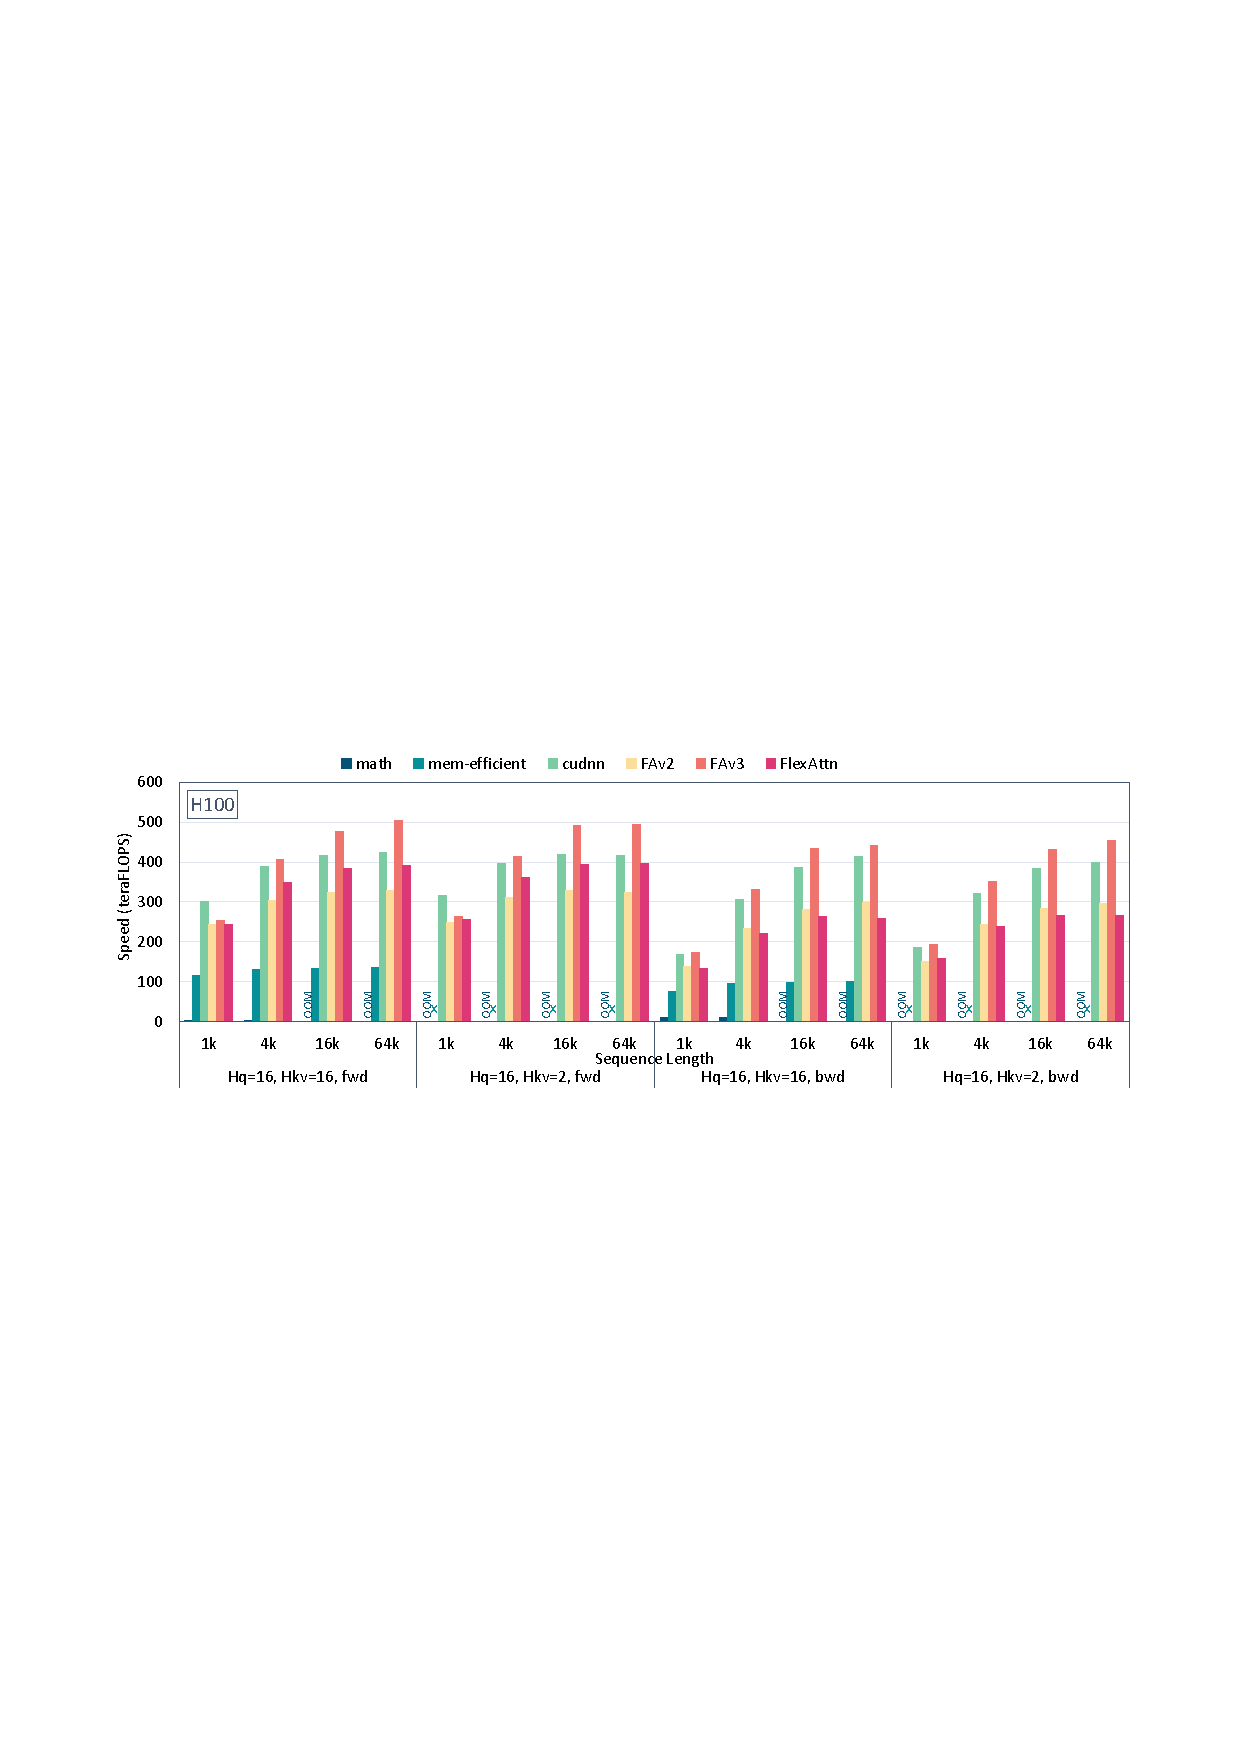
\includegraphics[width=0.9\textwidth]{graphs/causal_training_H100.pdf}
    \end{subfigure}
     \begin{subfigure}
         \centering
         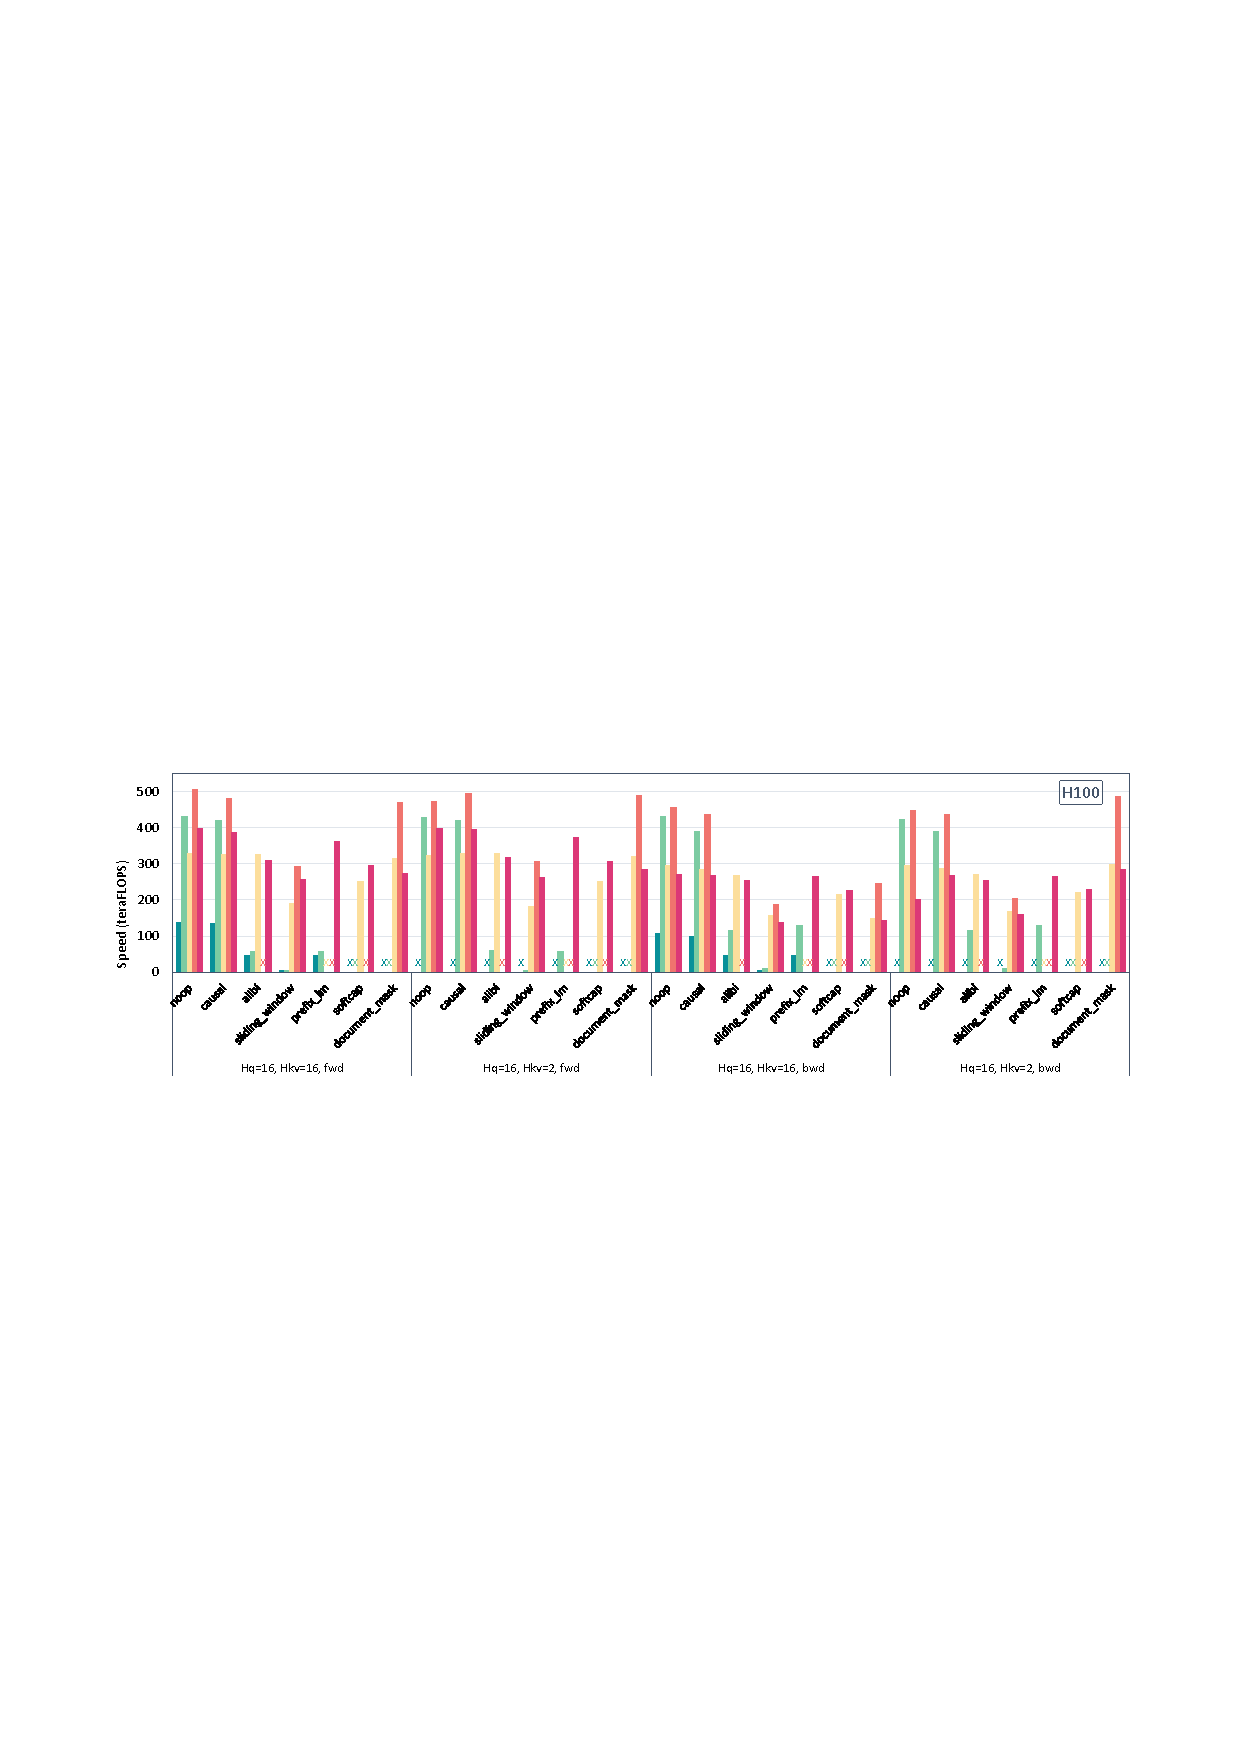
\includegraphics[width=\textwidth]{graphs/masks_training_H100.pdf}
    \end{subfigure}
    \caption{Attention Kernel Speed: Forward and Backward. \textbf{Top:} Causal Mask on QKV Length Ranging from 1k to 64k w/wo GQA. \textbf{Bottom: } Different Attention Variants on 16k-token-long QKV w/wo GQA.  }
    \label{fig:evaluation:benchmark_training}
\end{figure*}

\begin{figure*}[!h]
    \centering
  \begin{subfigure}
         \centering
         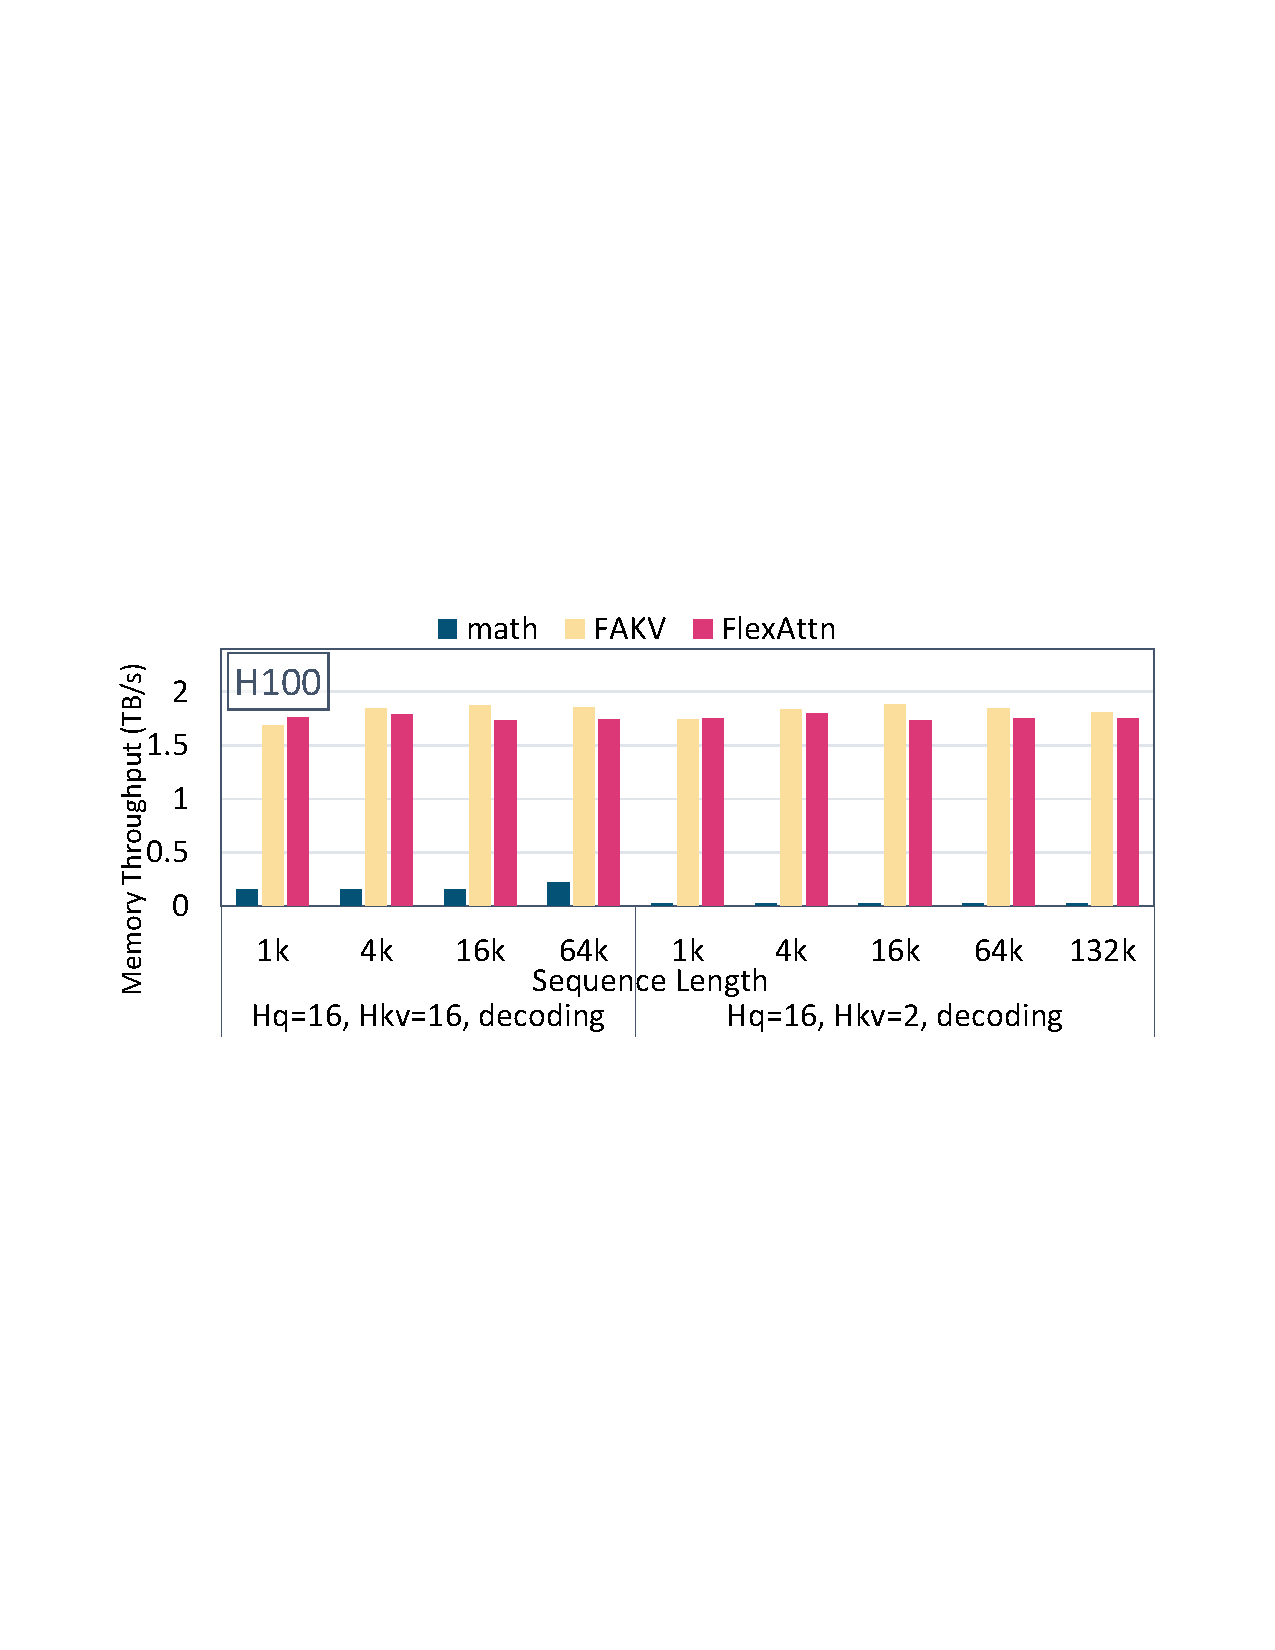
\includegraphics[width=0.49\linewidth]{graphs/noop_decoding_H100.pdf}
    \end{subfigure}
     \hfill
     \begin{subfigure}
         \centering
         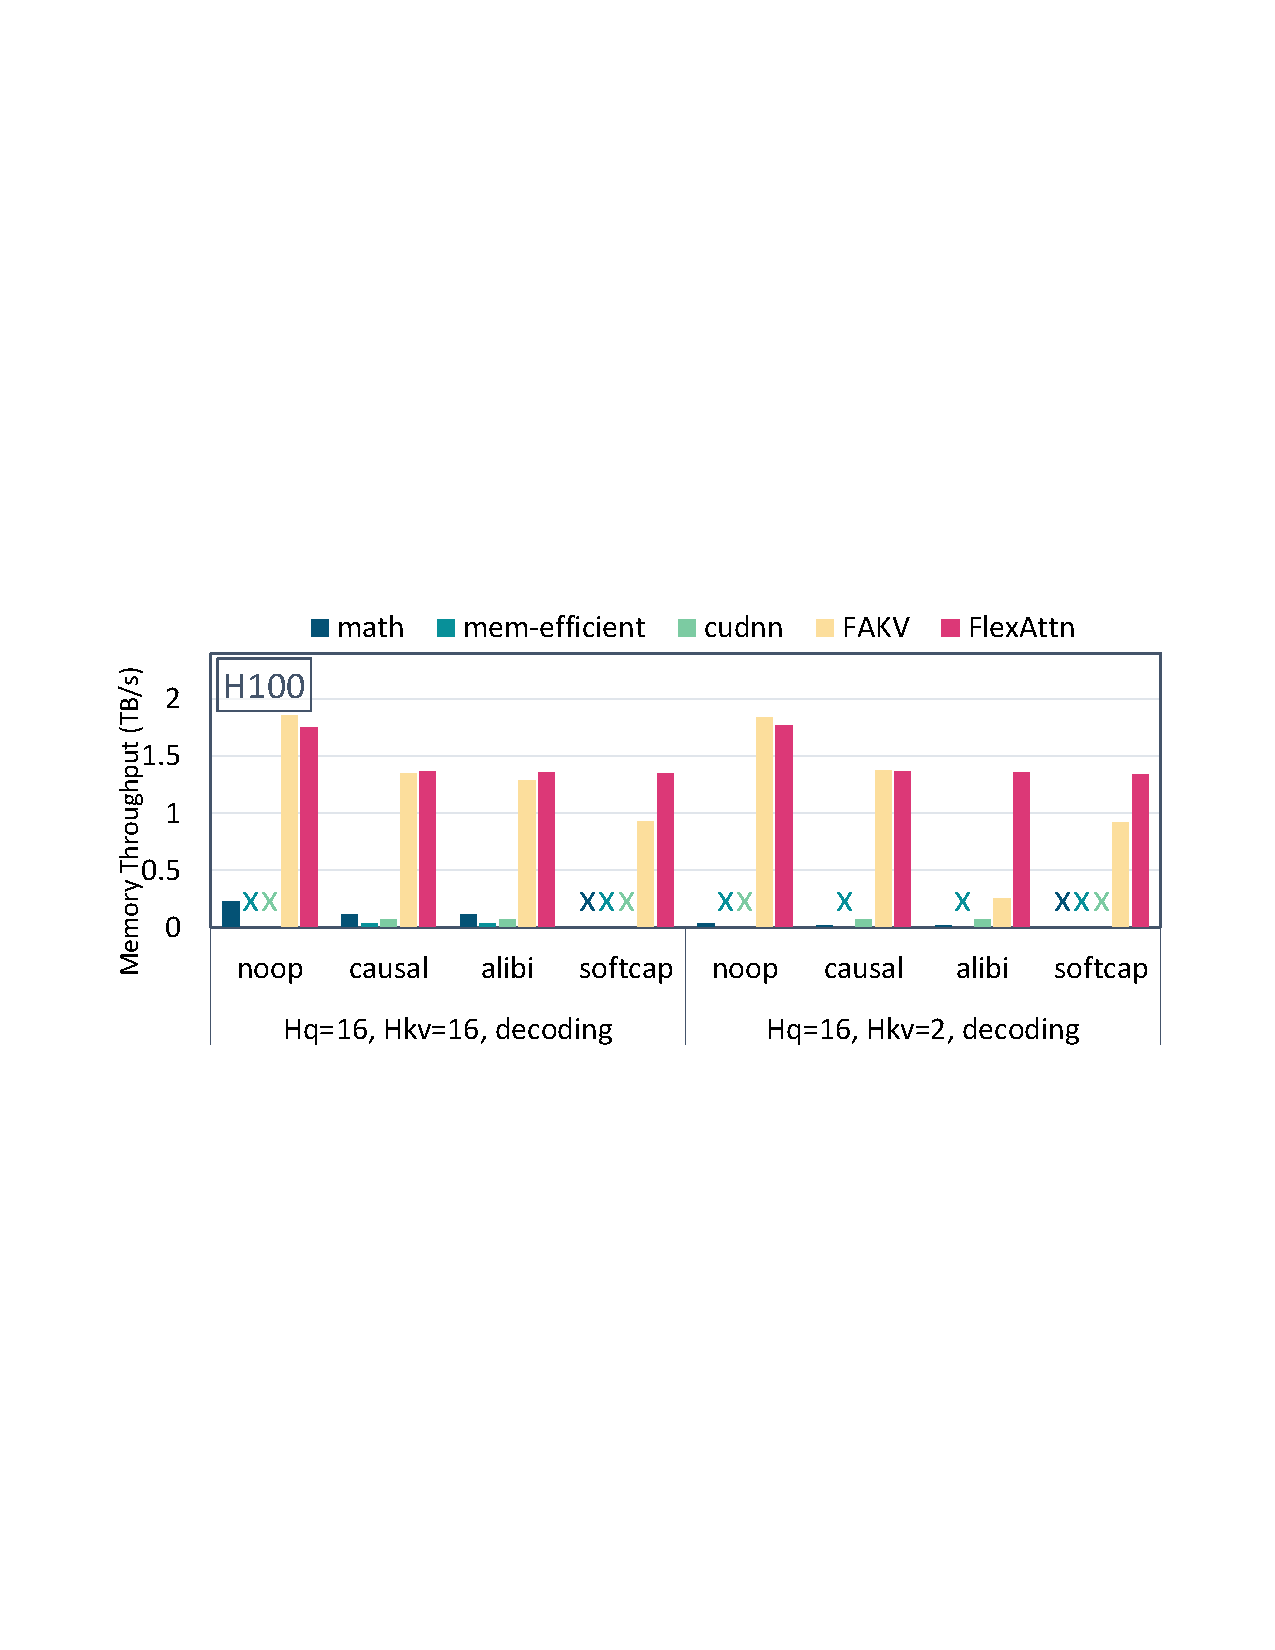
\includegraphics[width=0.49\linewidth]{graphs/decoding_score_mods_H100.pdf}
    \end{subfigure}
    \caption{Attention Kernel Speed: Decoding for 1 Query Token. \textbf{Left:} Classic Attention on KV Length Ranging from 1k to 132k w/wo GQA. \textbf{Right: } Different Attention Variants on 16k-token-long KV cache w/wo GQA.  }
    \label{fig:evaluation:benchmark_decoding}
\end{figure*}
\par 
\textbf{Inference Performance. } As shown in Figure \ref{fig:evaluation:benchmark_decoding}, for a query length of 1, \textit{FlexAttention} delivers decoding performance comparable to FlashDecoding ({\tt FAKV}), achieving a 0.93x-1.45x speedup, except one outlier: \textbf{\textit{FlexAttention} is 5.37x faster than {\tt FAKV} when using GQA with {\tt alibi}}. This is an example of the "software lottery", where {\tt FAKV} lacks manual optimization for GQA with {\tt alibi}, and its fallback solution provides only 1/5 of the optimal performance. In contrast, \textit{FlexAttention} maintains consistent performance for this combination without manual tuning. 
Due to page limit, we leave Neighborhood Attention results in Appendix A.1.

\par
\begin{figure}[!h]
    \centering
    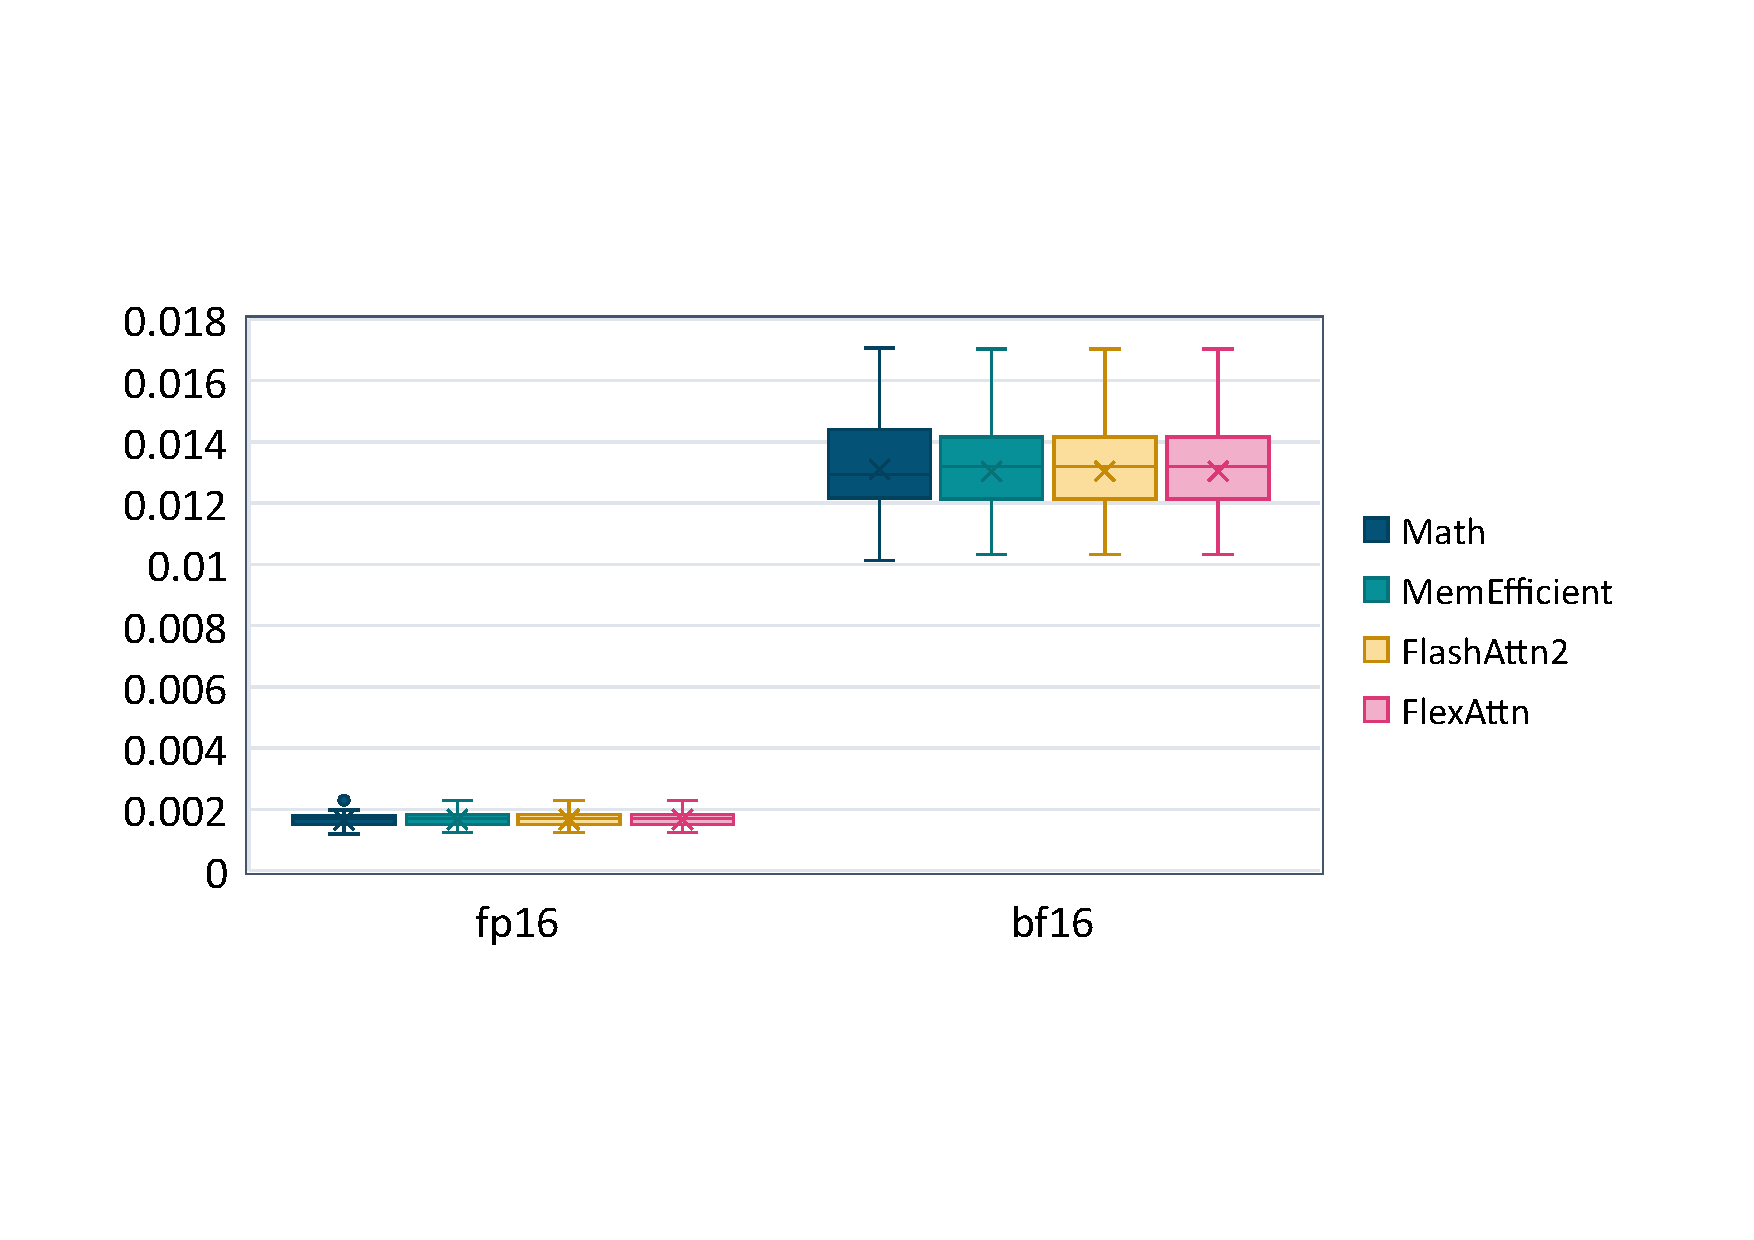
\includegraphics[width=0.9\linewidth]{graphs/errors1.pdf}
    \caption{Root-mean-square error (RMSE) of bf16 and fp16 attention output compared to fp64 golden result. }
    \label{fig:evaluation:numerics}
\end{figure}
\textbf{Numeric Accuracy. } \textit{FlexAttention} does not introduce additional numeric errors compared to our baselines. (Figure \ref{fig:evaluation:numerics})



\subsection{End-to-end Performance. }
\textit{FlexAttention} boosts end-to-end training performance by over 2.4x and inference performance by up to 2.04x, and this speedup scales well with sequence length. We replace SDPA with \textit{FlexAttention} in {\tt gpt-fast} and {\tt torchtune} libraries and evaluate performance on LLaMa3 and LLaMa3.1 models. We show that \textit{FlexAttention} integrates well with the PyTorch framework in {\tt gpt-fast} and {\tt torchtune}, enabling optimizations such as CUDA graphs, parameter freezing, and kernel fusion, same as SDPA. \par

\textbf{Training Performance of {\tt torchtune}. } We set up {\tt torchtune} to fine-tune LLaMa3-8B  on the Alpaca~\cite{alpaca} dataset. To efficiently process the input sequences of different lengths, {\tt torchtune} concatenates them into jagged long sequences of fixed length. This approach requires a document mask that allows each input sequence to attend to itself while ignoring its neighbors. SDPA utilizes a precomputed boolean mask of size $B\times N \times N$, where B is batch size and N is the sequence length. As shown in Figure \ref{fig:evaluation:torchtune}, the cost of accessing this boolean mask grows quadratically, leading to a 25\% decrease in the training throughput when the sequence length increases from 2k to 8k. In contrast, \textit{FlexAttention} employs a {\tt BlockMask} and a document ID tensor of size $B \times N$ and  scales effectively with sequence length. \par
\begin{figure}[!h]
    \centering
    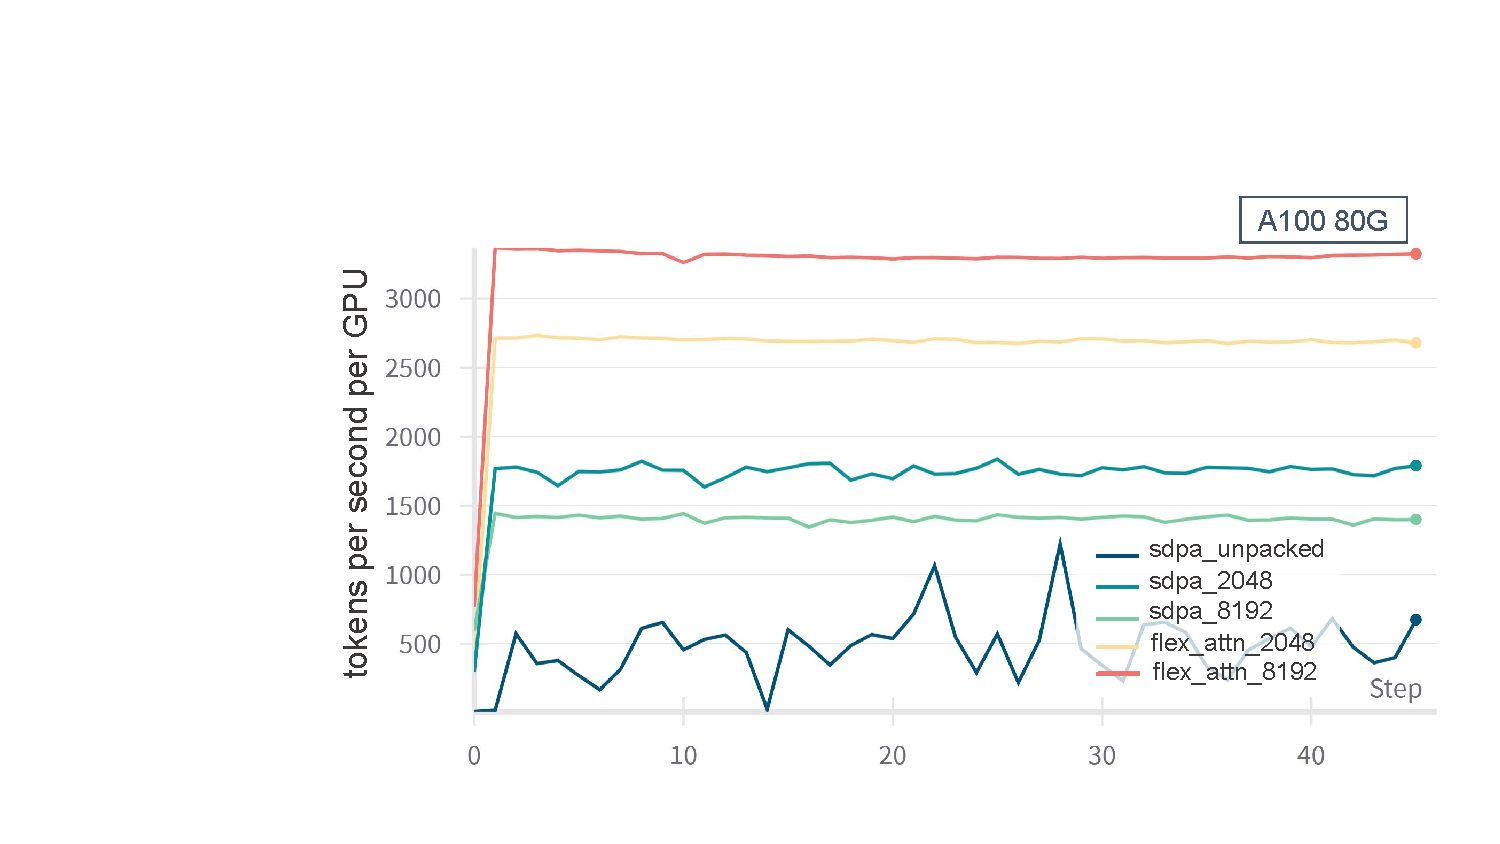
\includegraphics[width=\linewidth]{graphs/torchtune.pdf}
    \caption{{\tt torchtune} Training Throughput on llama3-8B. }
    \label{fig:evaluation:torchtune}
\end{figure}

\textbf{Inference Performance of {\tt gpt-fast}. } In Figure \ref{fig:evaluation:gpt-fast}, we show that \textit{FlexAttention} boosts LLaMa3.1-8B serving performance by 1.22x-2.04x, and LLaMa3.1-70B performance by 0.99x - 1.66x compared to SDPA. The speedup increases as context length grows and the attention kernel increasingly dominates the computation in each iteration. 

\begin{figure}[!h]
    \centering
    \begin{tabular}{@{}c@{}@{}c@{}}

    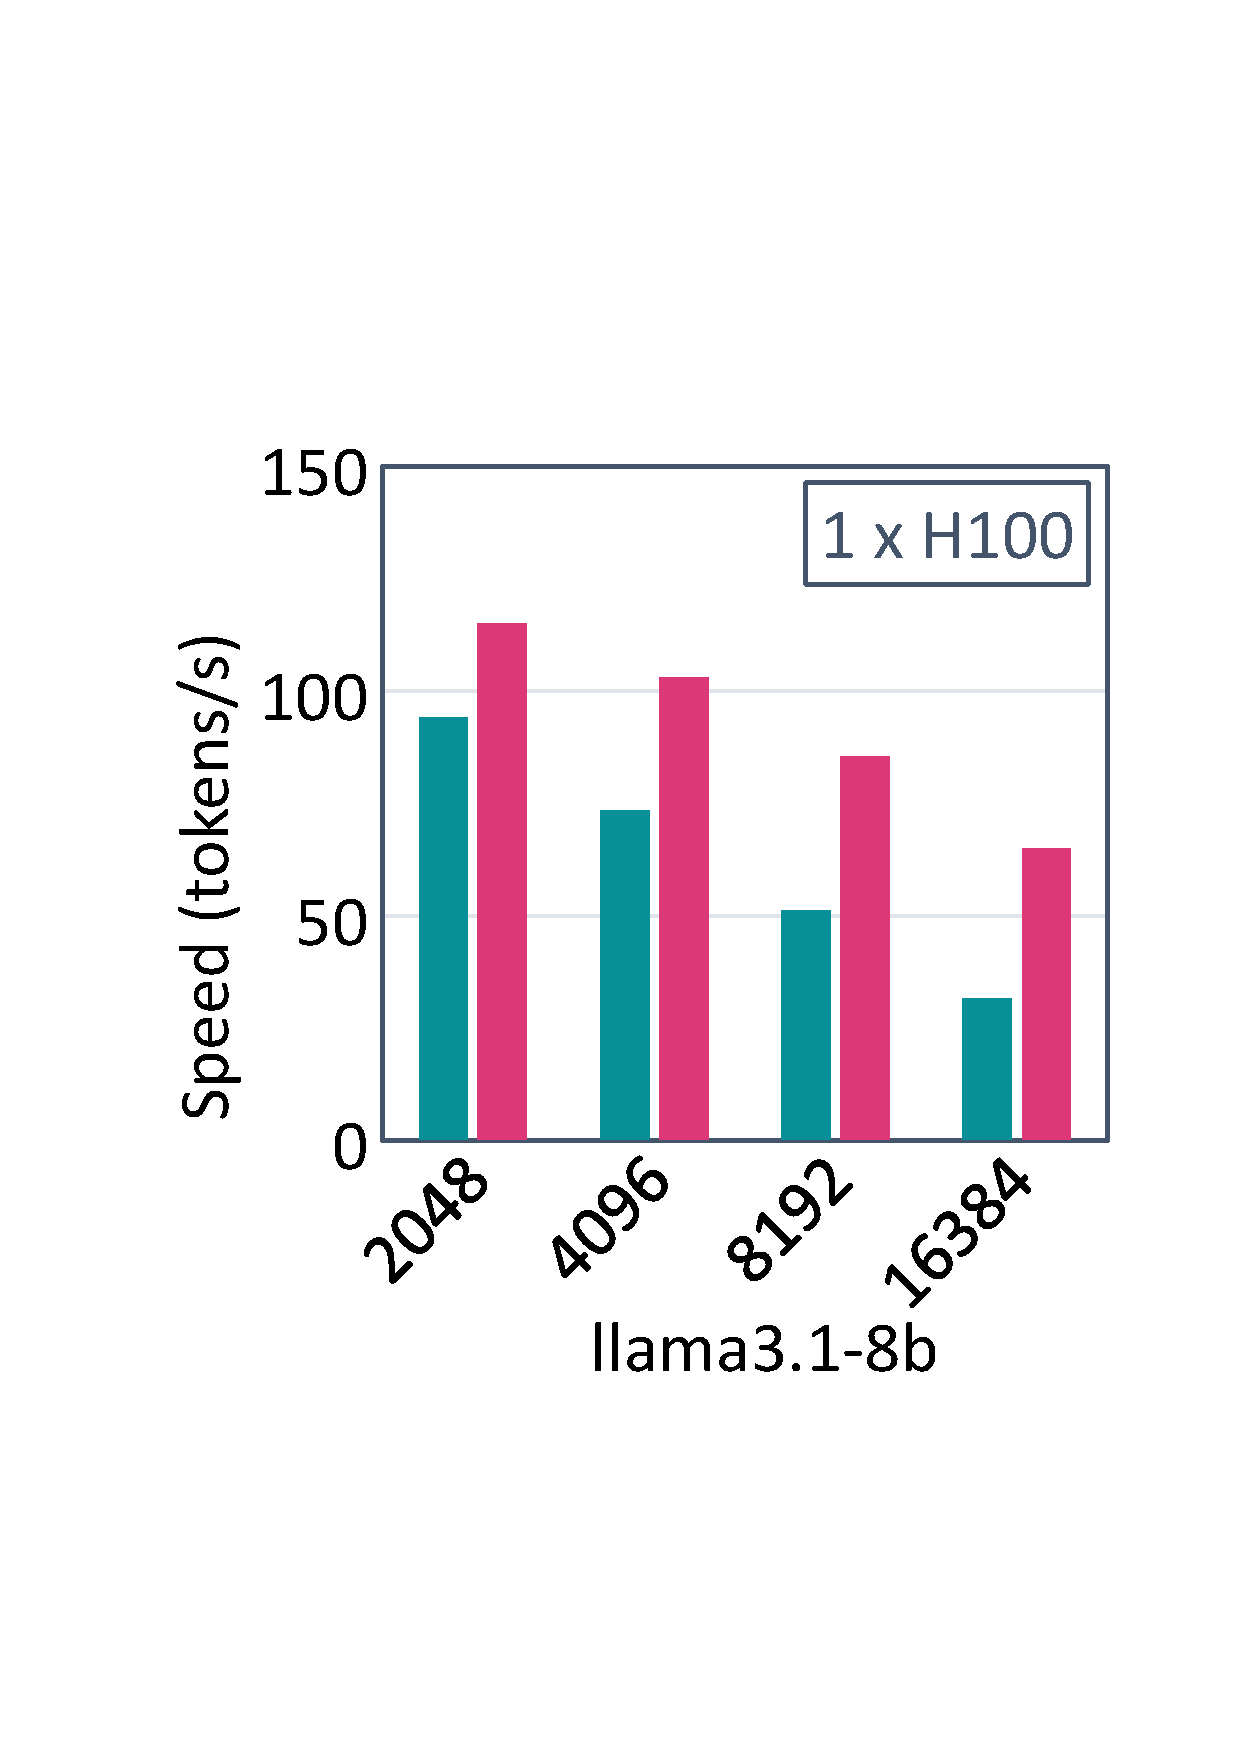
\includegraphics[width=0.51\linewidth]{graphs/gpt-fast-7b.pdf} & 
    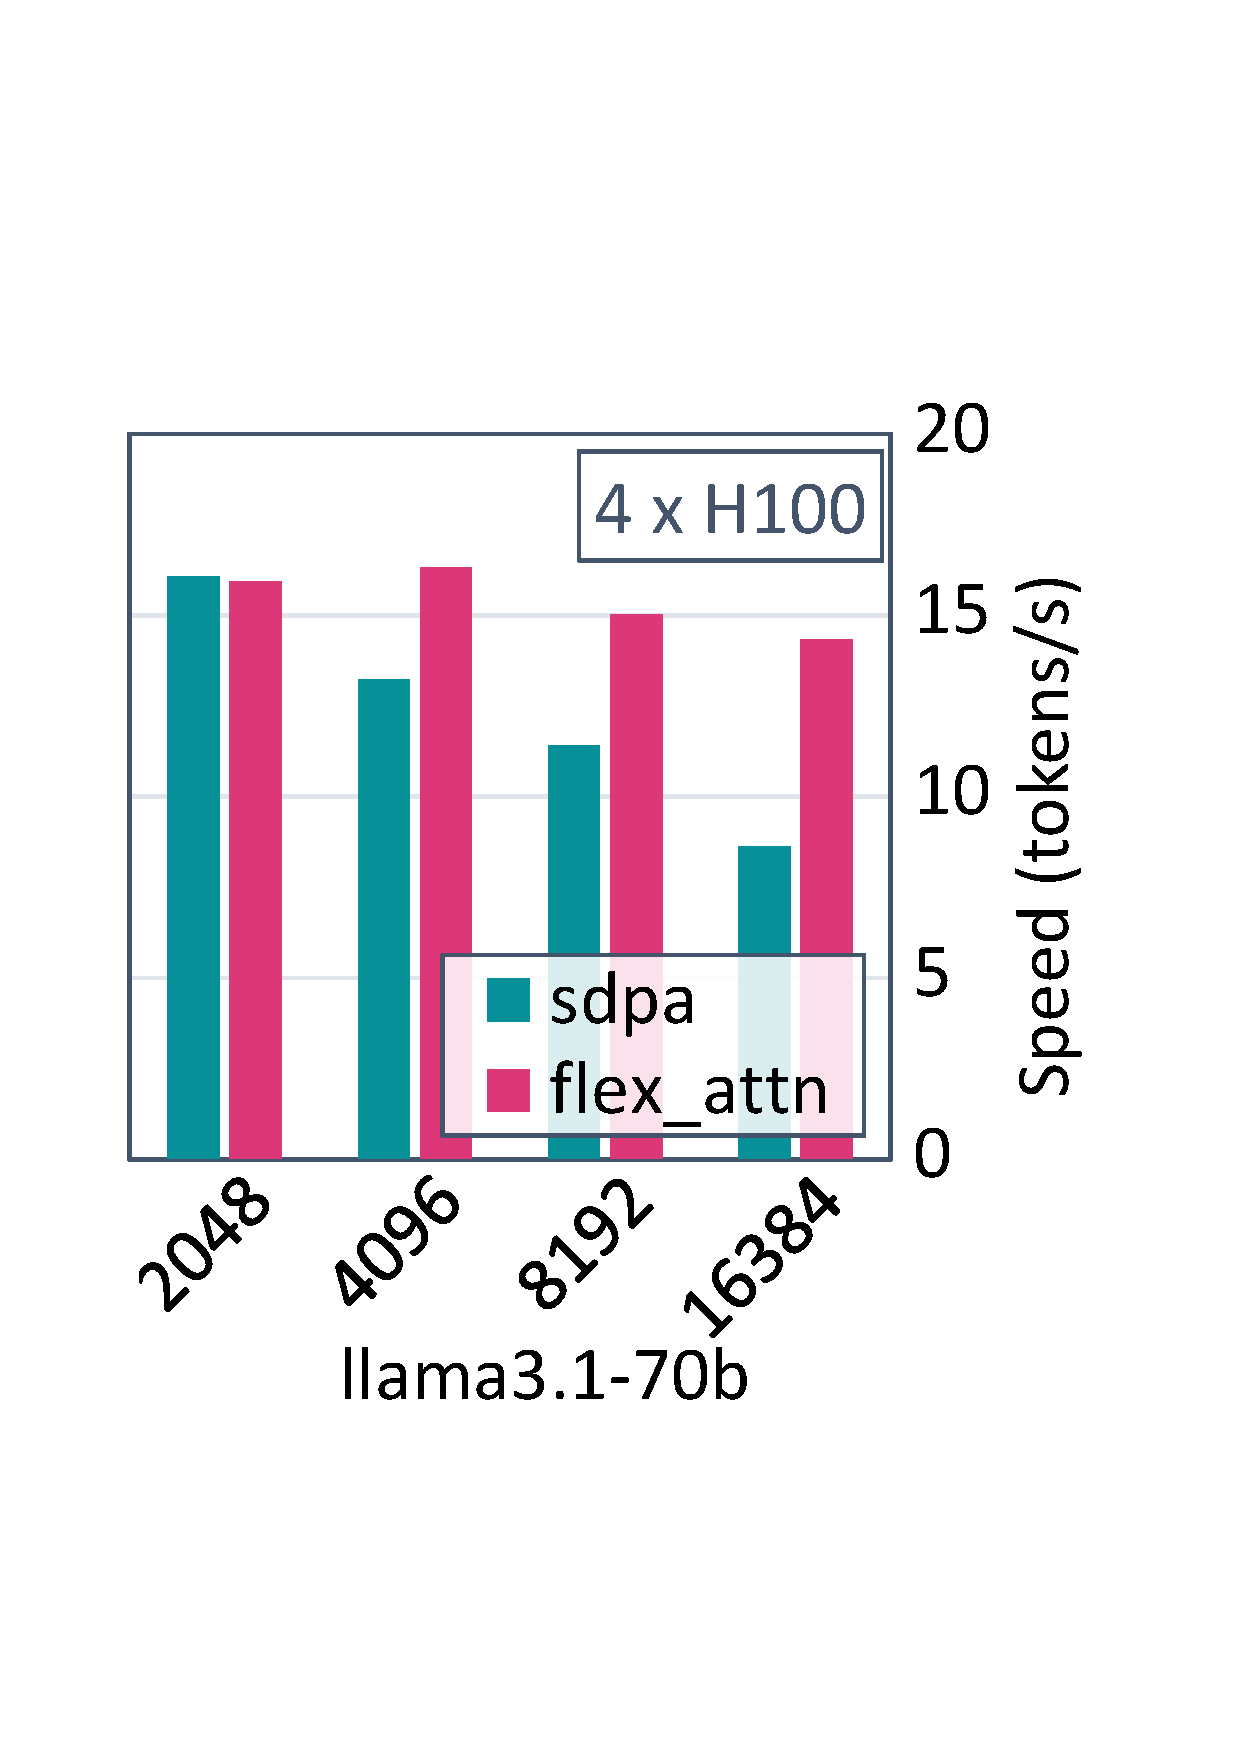
\includegraphics[width=0.48\linewidth]{graphs/gpt-fast-70b.pdf} 
    \\
    \end{tabular}
    \caption{{\tt gpt-fast} Inference Speed on LLaMa3.1-8B and 70B.}
    \label{fig:evaluation:gpt-fast}
\end{figure}


\subsection{Case Study: Paged Attention}

\begin{figure}[!h]
    \centering
  \begin{subfigure}
         \centering
         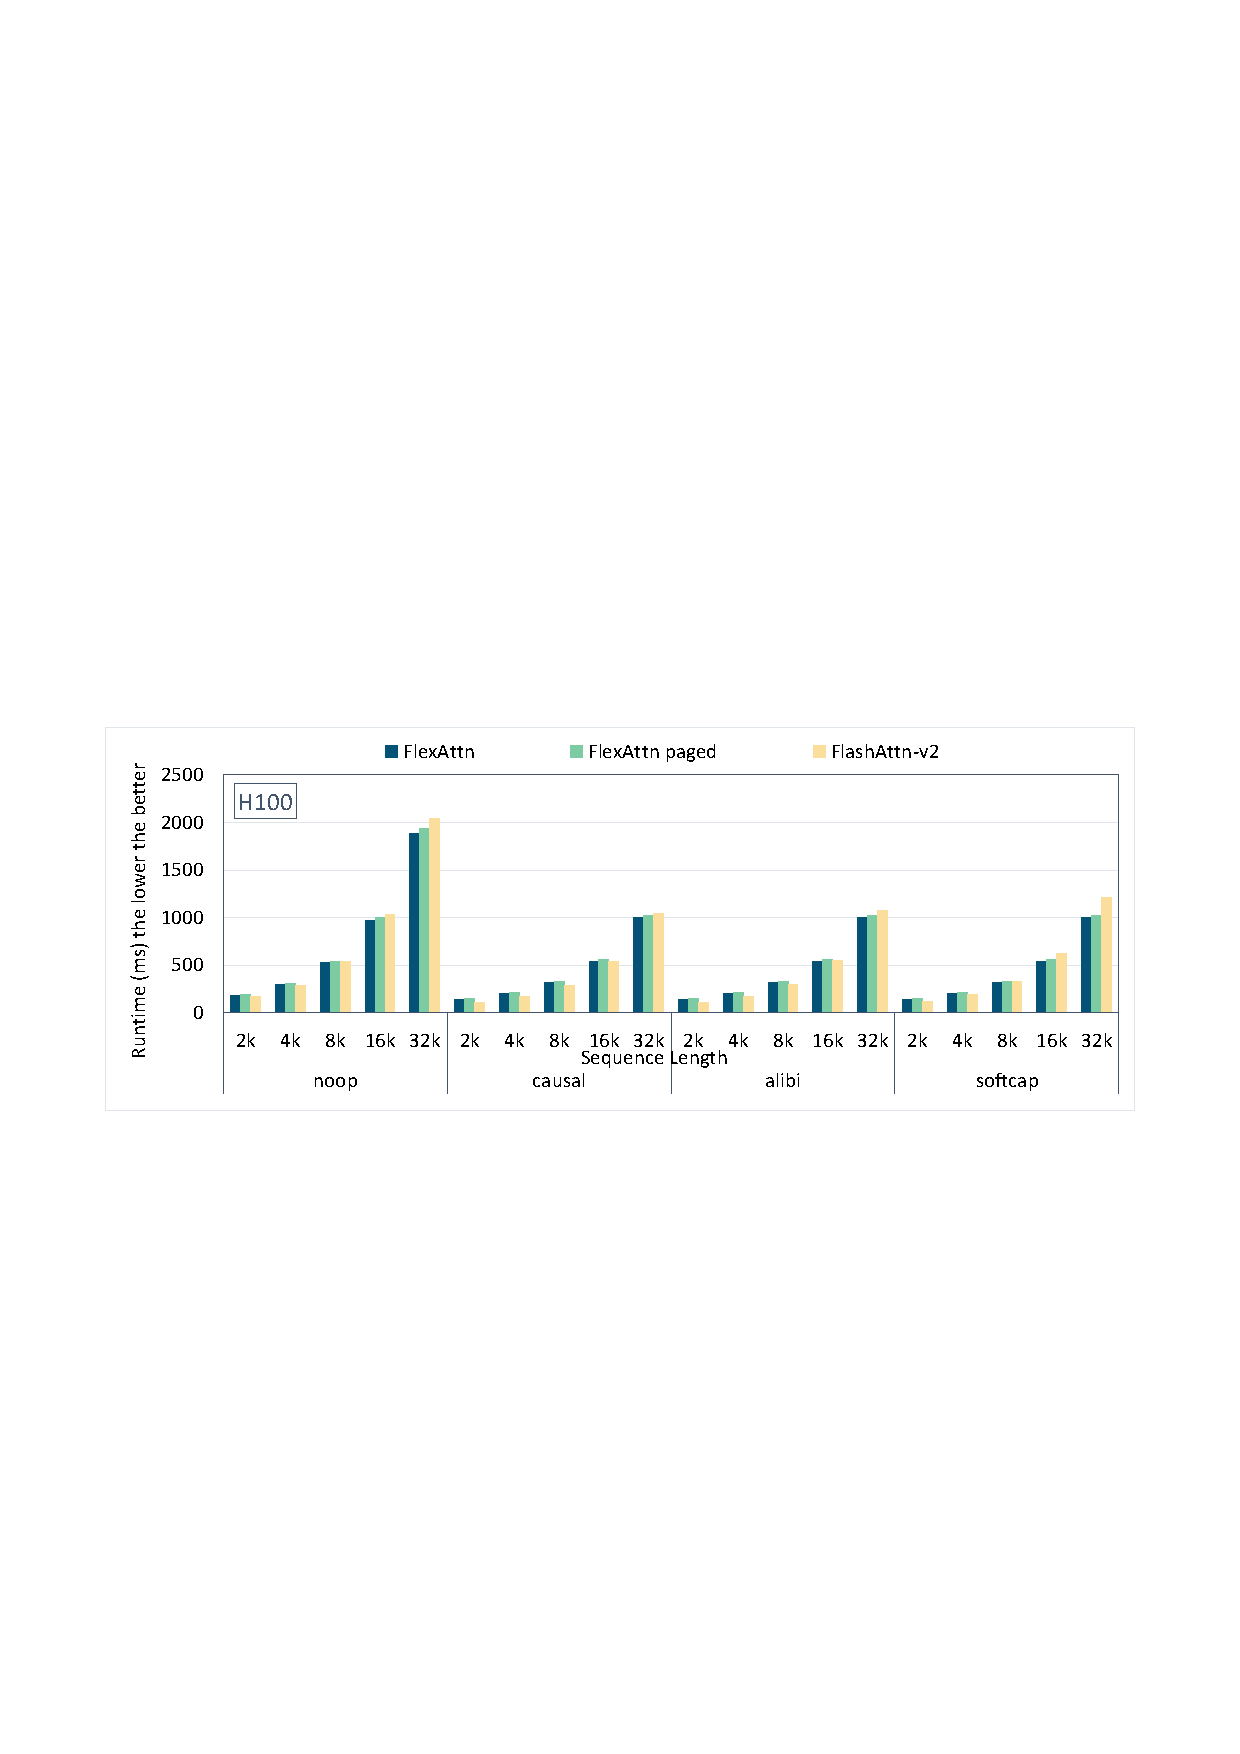
\includegraphics[width=\linewidth]{graphs/PagedSeqlen.pdf}
    \end{subfigure}
    % removed to save space
    %  \hfill
    %  \begin{subfigure}
    %      \centering
    %      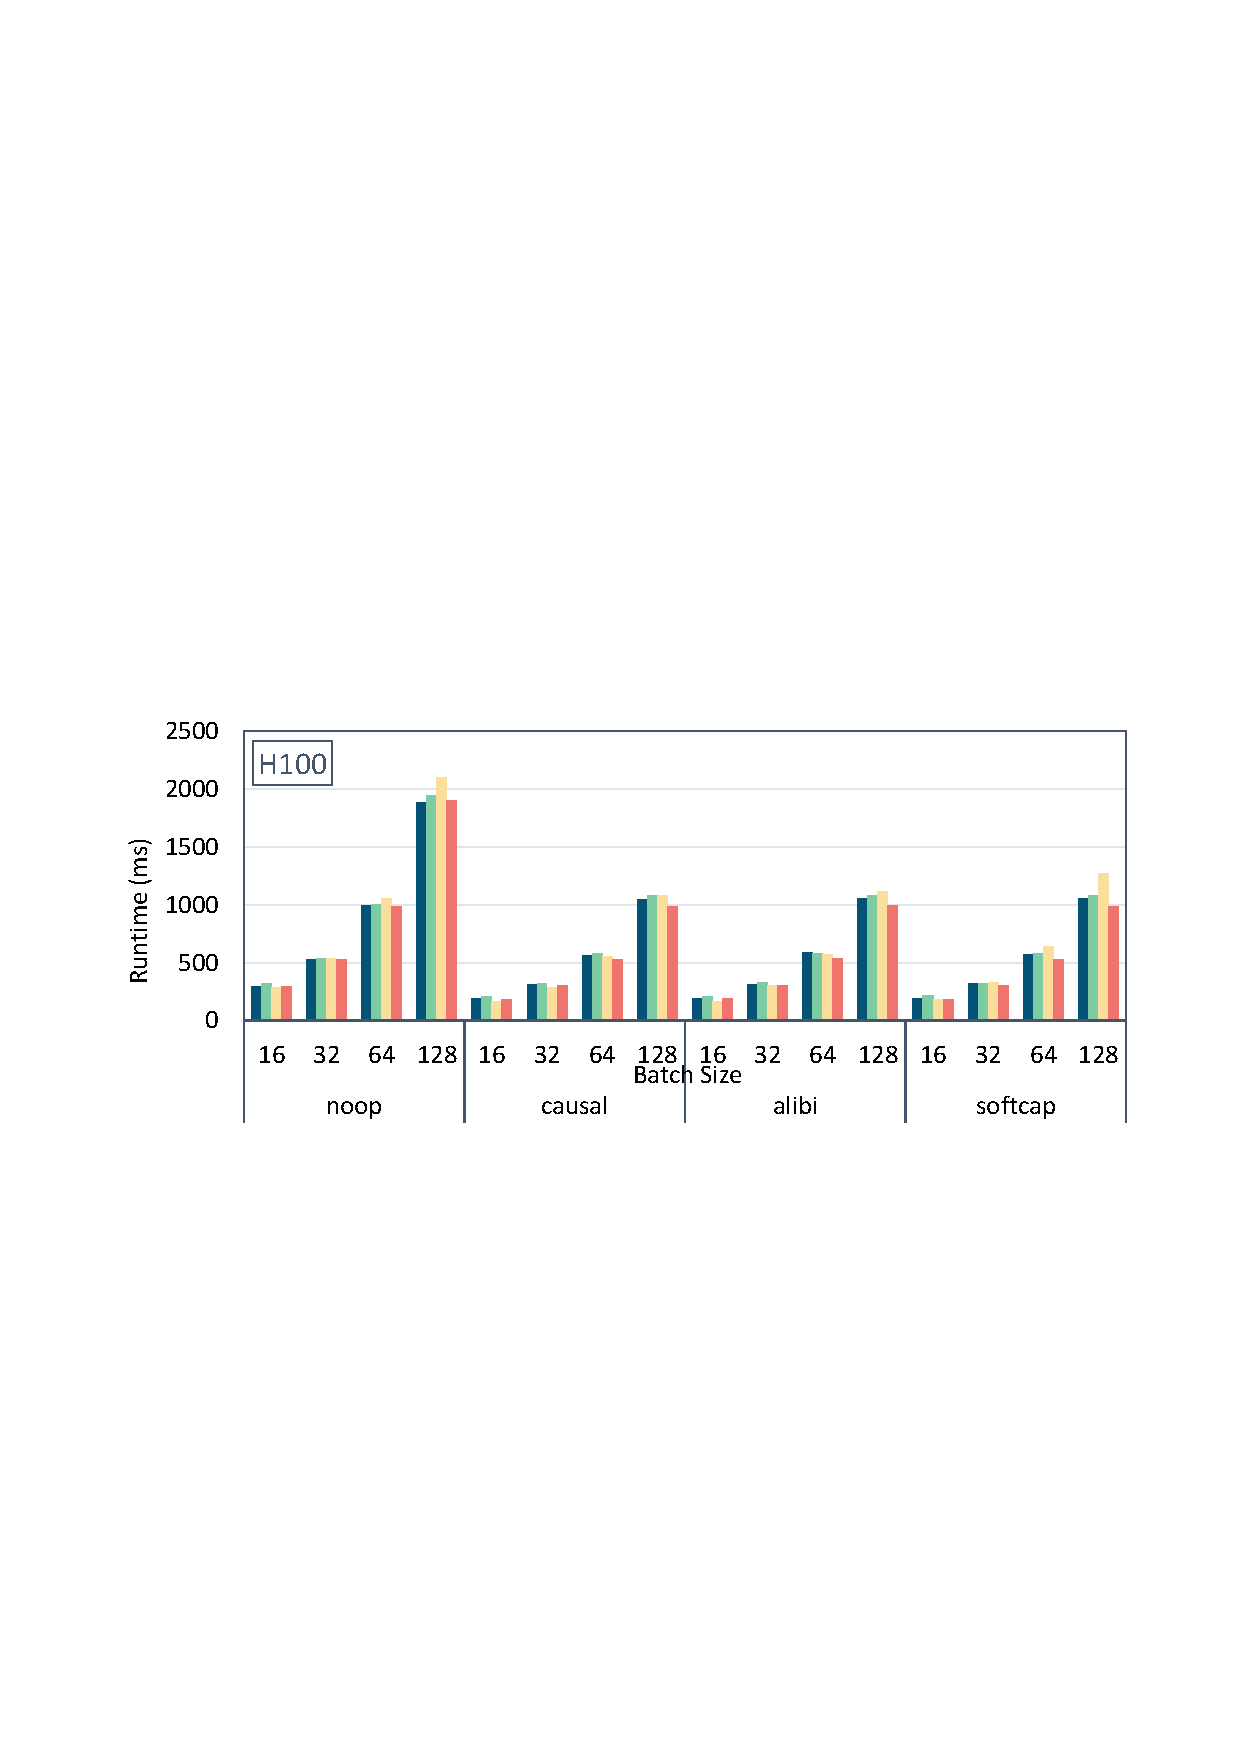
\includegraphics[width=\linewidth]{graphs/PagedBsz.pdf}
    % \end{subfigure}
    \hfill
    \begin{subfigure}
         \centering
         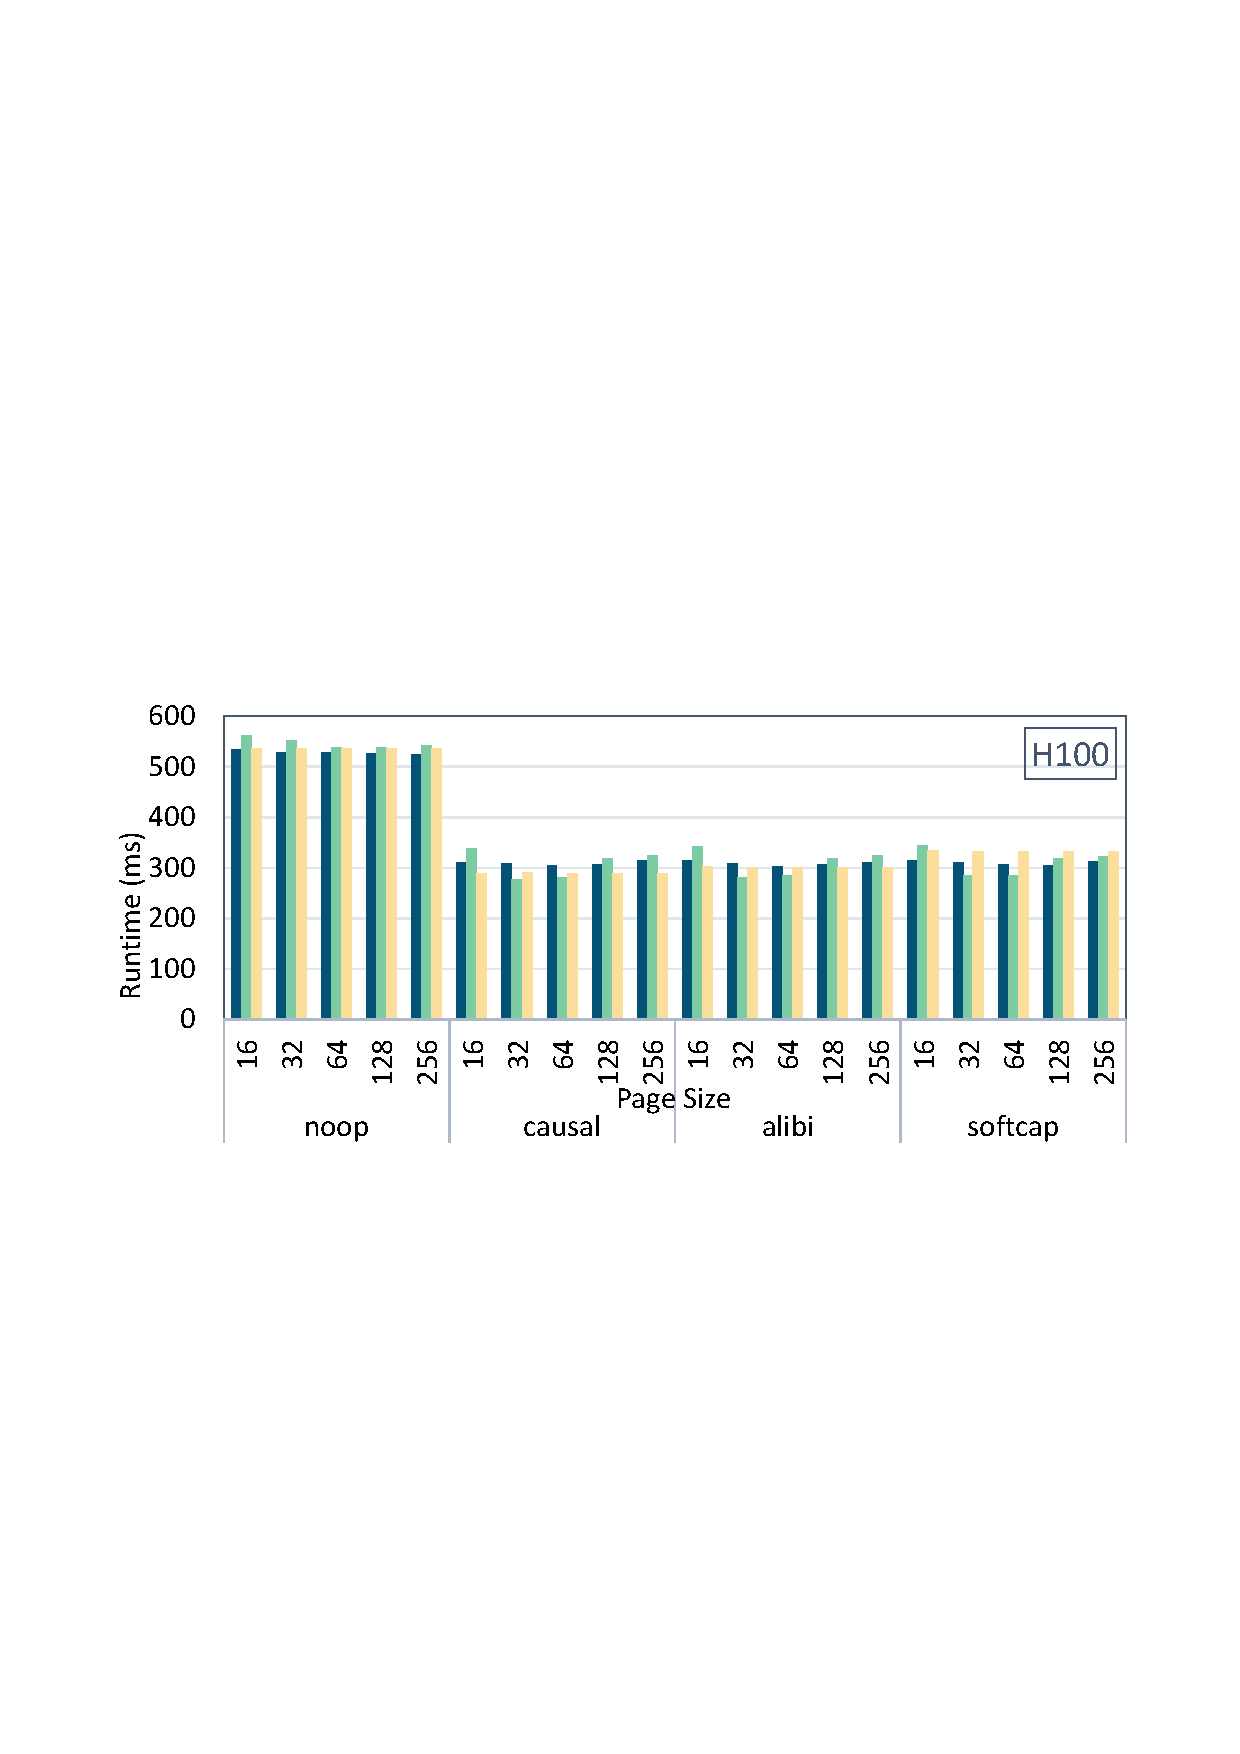
\includegraphics[width=\linewidth]{graphs/PagedPageSize.pdf}
    \end{subfigure}
    \caption{Runtime w/ and w/o paged attention (the lower the better). \textbf{Top:} Latency under diverse sequence length. \textbf{Bottom:} Latency under diverse page size.}
    \label{fig:evaluation:paged}
\end{figure}


While paged attention stores sentence requests of varying length in a compact physical KV cache, one major question is whether it would introduce high runtime overhead.
\autoref{fig:evaluation:paged}(a) shows runtime latency of flex attention with and without paged attention, as well as FlashAttn-v2.
We show runtime latency under changing sequence length, while keeping other dimension the same with batch size of 32, head dimension of 64, and number of heads as 16.
Overall, we observe less than 1\% runtime overhead on average when using \textit{FlexAttention} with paged attention, which is significantly smaller than the 20–26\% higher attention kernel overhead reported in vLLM~\cite{vLLM}.
The reason is that we do not introduce any kernel changes and rely on a fused indirect memory access to support \textit{FlexAttention} with paged attention.
Surprisingly, we even observe that \textit{FlexAttention} with paged attention is faster than FlashAttn-v2 without paged attention on large sequence lengths, which demonstrates the scalability of our design.

\autoref{fig:evaluation:paged}(b) demonstrates the impact from page size ranging from $16$ to $256$. Overall, we do not observe significant performance impact from changing page sizes.
Note that we manage physical KV cache in GPU global memory and do not swap memory to host disk, which mitigates the disk access overhead.





